\chapter{星际介质和恒星形成}
\section{星际尘埃和气体}
恒星和恒星之间实际上存在大量的各种尘埃和气体物质,虽然它们密度很低,但是由于星际间的大尺度距离,它们对星光的散射也是非常可观的。

星际介质对光强的减弱过程被称为\textbf{星际消光},如果将这种影响考虑进对星等的计算,则式\ref{eq:module}变为:
\begin{equation}
  m_\lambda=M_\lambda+5\log_{10}d-5+A_\lambda
\end{equation}

其中$A_\lambda \approx \tau_\lambda$表征星际介质对星等的影响,不同波长的光对应不同的值。

\paragraph{米氏散射理论}
给出任意尺寸的粒子的散射规律。当波长与尘埃直径相近时,散射截面$\sigma_\lambda \propto a^3/\lambda$,$a$为尘埃直径;当波长远小于尘埃直径时,$\sigma_\lambda \propto a^3/\lambda$。简单来说就是\textbf{星际介质对短波长的光散射能力更强},这会导致观测到的光中短波部分会被散射掉,使光看起来偏长波部分,这种现象称为星际红化


\paragraph{中性氢的21\,cm谱线}
如图\ref{fig:21cm},由于质子和电子都有内禀的自旋,两者同向自旋时比反向自旋,电子具有更高的能量,由于低能状态更加稳定,同向自旋的电子最终会变为反向自旋,并辐射出一个光子,这个光子的对应波长为21\,cm。同理,反向自旋的电子也可以吸收一个21\,cm波长的光子激发为反向自旋。

\begin{figure}[hbt]
  \centering
  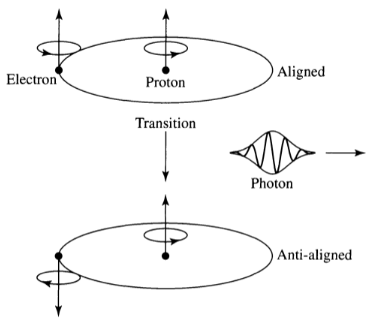
\includegraphics[width=6cm]{chapters/12/21cm}
  \caption{自旋示意图}
  \label{fig:21cm}
\end{figure}

观测上,可以通过21\;cm吸收线来测定中性氢的分布,因为其光深与中性氢柱密度成正比。

\section{原恒星的形成}
星际分子云也是引力束缚系统,前面\ref{virial}节提过稳定的引力束缚系统满足维里定律。反之如果系统的动能和引力不满足维里定理,就不稳定,尤其是当引力势能较大时,分子云就会塌缩。从实际来看,当\textbf{分子云的质量足够大时,一点微小的扰动就会造成分子云的塌缩},这个临界质量称为\textbf{金斯判据}:
\begin{equation}
  M_J\simeq\left({5kT\over G\mu m_H}\right)^{3/2}\left({3\over 4\pi \rho_0}\right)^{1/2}
\end{equation}

\section{主序前的演化}
随着分子云的塌缩,引力势能有一半转换为内能,升高原恒星的温度,还有一半会变成辐射。在塌缩过程中,原恒星在赫罗图\ref{fig:hayashi}上处于最右边近乎垂直的轨迹上,这条轨迹被称为\textbf{林忠四郎线轨迹},它代表的是流体静力学平衡的分界线,此时原恒星内部会产生大范围的对流来试图改变塌缩产生的温度梯度,达到流体静力学平衡。
\begin{figure}[hbt]
  \centering
  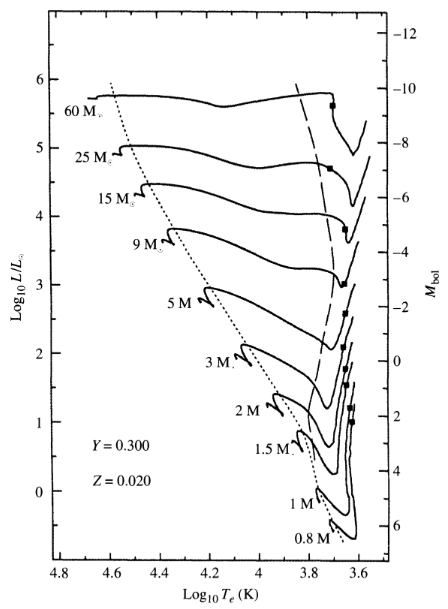
\includegraphics[width=10cm]{chapters/12/hayashi}
  \caption{主序前演化赫罗图}
  \label{fig:hayashi}
\end{figure}

原恒星会持续塌缩,直到温度高到能够平衡引力,而中心的温度是最高的,这时,不同质量的原恒星就会有不同的命运。

质量大于$0.08\,M_\odot$的原恒星在达到平衡前,中心温度会达到氢点燃的温度,开始进行核反应,这时恒星正式进入了主序阶段,该时刻被称为\textbf{零龄主序}。

而对于质量小于$0.08\,M_\odot$的原恒星,它们达到流体静力学平衡时,中心温度不够高,从而只能成为\textbf{褐矮星}。

\begin{figure}[hbt]
  \centering
  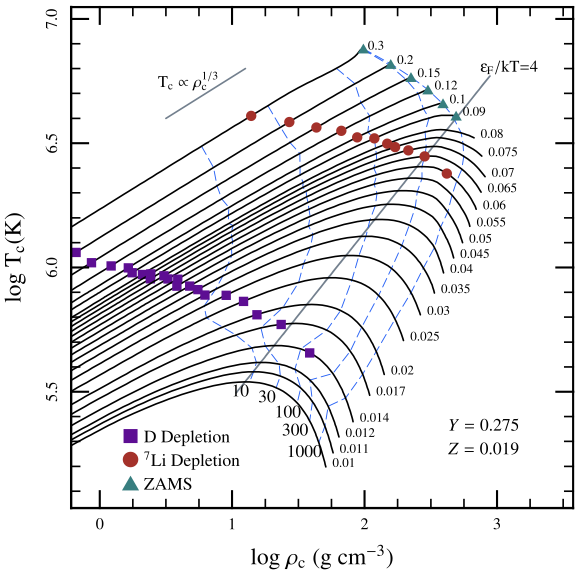
\includegraphics[width=12cm]{chapters/12/prems}
  \caption{不同质量原恒星主序前演化过程中的中心状态图,小于$0.08\,M_\odot$的原恒星无法进入零龄主序。}
  \label{}
\end{figure}
